\documentclass{article}
\usepackage{tikz,bm}
\usepackage[raggedrightboxes]{ragged2e}
\begin{document}
\begin{center}
  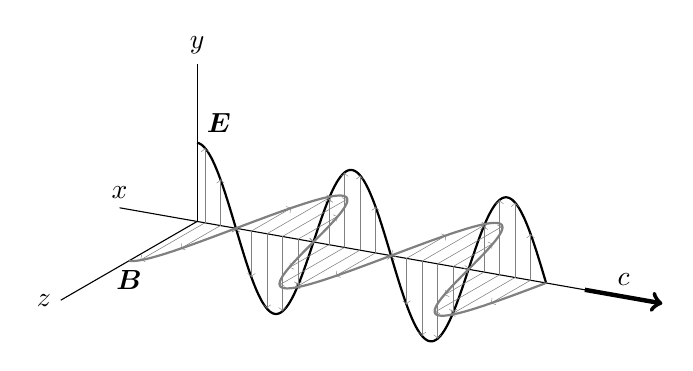
\begin{tikzpicture}[x={(-10:1cm)},y={(90:1cm)},z={(210:1cm)}]
    % Axes
    \draw (-1,0,0) node[above] {$x$} -- (5,0,0);
    \draw (0,0,0) -- (0,2,0) node[above] {$y$};
    \draw (0,0,0) -- (0,0,2) node[left] {$z$};
    % Propagation
    \draw[->,ultra thick] (5,0,0) -- node[above] {$c$} (6,0,0);
    % Waves
    \draw[thick] plot[domain=0:4.5,samples=200] (\x,{cos(deg(pi*\x))},0);
    \draw[gray,thick] plot[domain=0:4.5,samples=200] (\x,0,{cos(deg(pi*\x))});
    % Arrows
    \foreach \x in {0.1,0.3,...,4.4} {
      \draw[->,help lines] (\x,0,0) -- (\x,{cos(deg(pi*\x))},0);
      \draw[->,help lines] (\x,0,0) -- (\x,0,{cos(deg(pi*\x))});
    }
    % Labels
    \node[above right] at (0,1,0) {$\bm{E}$};
    \node[below] at (0,0,1) {$\bm{B}$};
  \end{tikzpicture}

  \begin{minipage}{.5\linewidth}
    \[
      c = \frac{E}{B}
    \]
    \begin{tabular}{r@{${}={}$}p{.8\linewidth}}
      $E$ & electric field amplitude \\
      $B$ & magnetic field amplitude (instantaneous values) \\
      $c$ & speed of light ($3\times10^8\mathrm{m/s}$) \\
    \end{tabular}
  \end{minipage}%
  \begin{minipage}{.5\linewidth}
    \[
      c = \frac{1}{\sqrt{\mu_0 \varepsilon_0}}
    \]
    \begin{tabular}{r@{${}={}$}p{.8\linewidth}}
      $\mu_0$ & magnetic permeability in a vacuum, $\mu_0 = 1.3\times10^{-6}\,\mathrm{N/A^2}$ \\
      $\varepsilon_0$ & electric permeability in a vacuum, $\varepsilon_0 = 8.9\times10^{-12}\,\mathrm{C^2/N m^2}$ \\
    \end{tabular}
  \end{minipage}
\end{center}
\end{document}